%!TEX root = ../main.tex

In this chapter, I first present examples of verification for the seven segment display example as well as the addone example. Secondly, an experiment has been conducted to gain further insight into program size and validation time. The experimental setup and results are introduced with the three properties \texttt{verification time}, \texttt{number of states} and \texttt{maximum resident set size}.
% TODO: Mention how to use taps if i keep it here.

\section{Seven Segments Display Example Validation}
The seven segments example has been presented in different parts throughout this thesis. An illustration of the entire translated unclocked seven segments network can be seen in Figure \ref{fig:cspm-network}. The SMEIL representation of the same network can be seen in Chapter \ref{chap:analysis} in Figure \ref{fig:smeil_network}.
The unclocked \cspm{} network consists of 12 different processes, all created so that not only the network is simulated correctly, but also so the monitor processes are placed correctly. The input is represented by a triangle, since it transpiles from an SME process to a \cspm{} channel it is not represented as a process in this network. Each of the dotted squares represents the network of synchronisations for each \texttt{time} processes, which in itself is a process in \cspm{}. For each network, we have the \texttt{time} processes and two monitor processes, for example, $H$, $M_{H_1}$ and $M_{H_2}$.
\\

% Errornous example
\begin{listing}
\begin{minted}[escapeinside=||, mathescape=true]{cspm_lexer.py:CSPmLexer -x}
channel clock_out_val : {0..131071}

channel hours_out_first_digit : {0..3}
channel hours_out_second_digit : {0..15}
    |$\vdots$|

Hours(hours_in) =
let
    hours = hours_in / 3600
    |$\vdots$|

Hours_out_first_digit_monitor(c) =
    c ? x -> if 0 <= x and x <= 2 then SKIP else STOP
Hours_out_second_digit_monitor(c) =
    c ? x -> if 0 <= x and x <= 9 then SKIP else STOP

\end{minted}
\caption{Example of an erroneous version of the \texttt{Hours} process from the \cspm{} seven segment display example seen in Listing~\ref{lst:smeil} and in Listing~\ref{lst:cspm} in the appendix.}
\label{lst:cspm_error}
\end{listing}

In order to show that the verification is accurate, the example in Listing~\ref{lst:cspm_error} contains an error that results in FDR4 failing the verification. In Listing~\ref{lst:cspm_error} the example is only able to handle an input that is below 24 hours. This is because the calculation in the \texttt{Hours} process does not handle the wrap around at the 24\textsuperscript{th} hour. This means that if the input represents more than 24 hours, the assertions will fail in FDR4 because one seven segment display suddenly has to display two digits instead of one. An example of such could be the input \texttt{131071}, which represents 36 hours, 24 minutes and 31 seconds, or 1 day, 12 hours, 24 minutes and 31 seconds. When trying to assert the code from Listing~\ref{lst:cspm_error} in FDR4, the assertion fails. The counterexample, provided by FDR4, shows that the number 3 is communicated on \texttt{hours\_out\_first\_digit}, which is not allowed according to the monitor process on lines 12 and 13 in Listing~\ref{lst:cspm_error}.\\

This example of failure shows how verifying the solution with a tool like FDR4 actually catches errors that the developer might have overseen. In this case, the error is simply corrected by adding \texttt{\% 24} on the end of line 9 in Listing~\ref{lst:cspm_error} and can be seen corrected in Listing~\ref{lst:cspm} in the appendix at line 15. Now when we try to assert the example in FDR4, it passes. By using modulo on the result, we ensure that we still get the accurate time of day, no matter how many full days the input represents.
The full SMEIL and \cspm{} code for the unclocked seven segment display example can be seen in Listing~\ref{lst:smeil} and in Listing~\ref{lst:cspm} in the appendix.

\begin{figure}[!ht]
  \centering
  \begin{tikzpicture}
    \node [mytriangle] (I) at (0, 0) {$I$};

    %%%%

    \node [mycircle, above right=25ex and 25ex of I] (H) {$H$};

    \node [mysquare, above right=1.5ex and 25ex of H] (H_d1) {$D_{H_1}$};
    \node [mysquare, below right=1.5ex and 25ex of H] (H_d2) {$D_{H_2}$};
    \node [mycircle, above right=3ex and 7.5ex of H] (H_m1) {$M_{H_1}$};
    \node [mycircle, below right=3ex and 7.5ex of H] (H_m2) {$M_{H_2}$};
    \node [draw, red, thick, dotted, fit=(H)(H_m1)(H_m2), inner sep=0.5cm] {};
    \node [right=15ex of H, red] {$N_{hours}$};

    \draw [myarrow, smooth] (I) to[out=0, in=180] (H);

    \draw [myarrow, smooth] (H) to[out=0, in=180] coordinate[midway, black!50, draw, shape=circle, inner sep=0pt, minimum size=5pt](H_mp1) (H_d1);
    \draw (H_m1) -- (H_mp1)  [black!50];
    \draw [myarrow, smooth] (H) to[out=0, in=180] coordinate[midway, black!50, draw, shape=circle, inner sep=0pt, minimum size=5pt](H_mp2) (H_d2);
    \draw (H_m2) -- (H_mp2)  [black!50];

    %%%%

    \node [mycircle, right=23.2ex of I] (M) {$M$};

    \node [mysquare, above right=1.5ex and 25ex of M] (M_d1) {$D_{M_1}$};
    \node [mysquare, below right=1.5ex and 25ex of M] (M_d2) {$D_{M_2}$};
    \node [mycircle, above right=3ex and 7.5ex of M] (M_m1) {$M_{M_1}$};
    \node [mycircle, below right=3ex and 7.5ex of M] (M_m2) {$M_{M_2}$};
    \node [draw, red, thick, dotted, fit=(M)(M_m1)(M_m2), inner sep=0.5cm] {};
    \node [right=15ex of M, red] {$N_{minutes}$};

    \draw [myarrow, smooth] (I) to[out=0, in=180] (M);

    \draw [myarrow, smooth] (M) to[out=0, in=180] coordinate[midway, black!50, draw, shape=circle, inner sep=0pt, minimum size=5pt](M_mp1) (M_d1);
    \draw (M_m1) -- (M_mp1)  [black!50];
    \draw [myarrow, smooth] (M) to[out=0, in=180] coordinate[midway, black!50, draw, shape=circle, inner sep=0pt, minimum size=5pt](M_mp2) (M_d2);
    \draw (M_m2) -- (M_mp2)  [black!50];

    %%%%

    \node [mycircle, below right=24.5ex and 24.5ex of I] (S) {$S$};

    \node [mysquare, above right=1.5ex and 25ex of S] (S_d1) {$D_{S_1}$};
    \node [mysquare, below right=1.5ex and 25ex of S] (S_d2) {$D_{S_2}$};
    \node [mycircle, above right=3ex and 7.5ex of S] (S_m1) {$M_{S_1}$};
    \node [mycircle, below right=3ex and 7.5ex of S] (S_m2) {$M_{S_2}$};
    \node [draw, red, thick, dotted, fit=(S)(S_m1)(S_m2), inner sep=0.50cm, inner ysep=0.5cm] {};
    \node [right=15ex of S, red] {$N_{seconds}$};

    \draw [myarrow, smooth] (I) to[out=0, in=180] (S);

    \draw [myarrow, smooth] (S) to[out=0, in=180] coordinate[midway, black!50, draw, shape=circle, inner sep=0pt, minimum size=5pt](S_mp1) (S_d1);
    \draw (S_m1) -- (S_mp1)  [black!50];
    \draw [myarrow, smooth] (S) to[out=0, in=180] coordinate[midway, black!50, draw, shape=circle, inner sep=0pt, minimum size=5pt](S_mp2) (S_d2);
    \draw (S_m2) -- (S_mp2)  [black!50];
  \end{tikzpicture}
  \caption{A seven segment display clock network in \cspm{}. $I$ represents the input channel. $N_{hours}$, $N_{minutes}$ and $N_{seconds}$ represent the network processes with $H$, $M$ and $S$ as the \texttt{time} processes. The results from the \texttt{time} processes are communicated to the displays. The displays are represented by a square since they are not actual \cspm{} processes. Each display communication also has a monitor process which assert the legal communication values.}
  \label{fig:cspm-network}
\end{figure}
\subsection{Clocked Seven Segments Display Example}
The internal states do not change between clock cycles in the seven segment display example, and so it can be verified with the unclocked version of TAPS. However, it was interesting to see how the network could be translated to a clocked structure. The full \cspm{} code of the clocked seven segment display example can be seen in Listing \ref{lst:clocked_seven_seg_example} in the appendix. %TODO: Add stuff here about appendix.
The example is very similar to the unclocked version, however, the processes all synchronise on the \texttt{sync} process as described in Chapter \ref{chap:clock}. Each \texttt{time} process synchronises, then reads a value from the input range, then synchronise again before performing the computation. Afterwards, the value is written to the output channel which the monitor process reads from, just like the unclocked seven segments example. This clocked example is a bit different than the \texttt{addone} example introduced in Chapter \ref{chap:clock} because there is no buffers in the clocked seven segment display network. This is because there are no synchronised processes communicating and therefore there are no need for buffers. This means that the network is not as complex as it could have been if buffers had been added.
Because the seven segment display network does not keep values between each clock cycle there is no need to verify more than one clock cycle and so when the \texttt{Clock} process terminates after one clock cycle, the network will behave the same as the unclocked seven segment display network. By looking through the FDR4 traces and the ProBE visualisations, it is clear that the two networks are equivalent in terms of verification and failures.
\section{Addone Example Validation}
The \texttt{addone} example has been introduced in Chapter \ref{chap:clock} and an illustration of the clocked network with its monitor processes can be seen in Figure \ref{fig:addone_clocked_monitor} in the same chapter. As explained, the \texttt{addone} example does not translate well in the initial version of TAPS and therefore the clocked version was created.
The difference between verifying the \texttt{addone} network with a clocked and unclocked network is that FDR4 is only able to verify one internal state in the unclocked version whereas it is able to verify more than one internal state in the clocked version. The possibility of verifying different internal states suits this cyclic network perfectly.\\

The \texttt{addone} example differs from the seven segment example in that it does not require an input range because the cyclic network is instantiated with initial values instead of a data generator process. The cyclic structure of the \texttt{addone} example causes the values to circulate and increase indefinitely if not restricted. It is not possible to represent an indefinite amount of values on hardware buses and therefore it must be restricted to a specific bit size. If the network is not restricted to specific values, the verification will be based on the values from the simulation of the SMEIL network, even though the network does not fail if values increase further.  This can cause an unnecessary failure in the verification. \\

If an SMEIL simulation of an unrestricted \texttt{addone} network results in the internal values reaching 20 and the FDR4 verification verifies more clock cycles than the SMEIL simulation, this would cause the values of the FDR4 verification to exceed the observed values, which would cause FDR4 to fail the verification. It is, therefore, necessary that the user makes an informed choice as to the number of clock cycles to simulate in SMEIL but also to verify in FDR4. The number of simulated clock cycles and FDR4 verified clock cycles do not have to be equal, but in some cases, it might be the obvious choice. \\

As mentioned, the \texttt{addone} example should be restricted and so a \texttt{\% 5} statement has been added to the computation in the \texttt{add} process to avoid the value becoming larger than 5. Listing \ref{lst:addone_mod_example} shows the simulated \texttt{addone} network with the restriction added in the \texttt{add} process. Besides the restriction, this example is identical to the example in Listing \ref{lst:addone_smeil_example} in Chapter \ref{chap:clock}.
With this enhanced example, the SMEIL simulation provides reasonable observed values which can be used for the verification in FDR4. In Listing \ref{lst:cspm_addone_restricted} a subset of the translated \texttt{addone} example can be seen which includes the restriction.
% TODO: Add something about where the entire code can be seen
After 10 clock cycles, the value becomes larger than 5, but the restriction ensures that the verification will succeed even if verified more than 10 clock cycles. The value will simply wrap around and continue at 0. If the restriction is removed and FDR4 verifies more than 10 clock cycles, the verification fails as expected. \\

This example is somewhat awkward to verify with FDR4 since it does not take advantage of the state space exploration that FDR4 provides. The lack of an input range for the system means that for each clock cycle a new state machine is verified, but only the internal values change. In this example, FDR4 only verifies the relation between internal values for each clock cycles with no external influence. The advantage of the clocked structure is that values, which might cause failures after a certain amount of clock cycles, are now possible to verify, which was not possible with the initial version of TAPS. \\

It is easy to see that this example never fails with the added restriction, but the example clearly introduces the clocked version of TAPS and how it is possible to verify clocked networks in FDR4 and therefore it still provides value to this thesis.

\begin{listing}
\begin{minted}{smeil_lexer.py:SMEILLexer -x}

proc id (in input)
    bus output {
        val: u4 = 0 range 0 to 4;
    };
    var from_add: u4 range 0 to 4;
{
    from_add = input.val;
    output.val = from_add;
}

proc add (in input, const constant)
    bus output {
        val: u4 = 0 range 0 to 4;
    };
    var from_id: u4 range 0 to 4;
{
    from_id = (input.val + constant) % 5;
    output.val = from_id;
}

network addone_network ()
{
    instance id of id(add.output);
    instance add of add(id.output, constant: 1);
}
\end{minted}
\caption{The restricted SMEIL network \texttt{addone\_network} similar to the example in Listing \ref{lst:addone_smeil_example}.}
\label{lst:addone_mod_example}
\end{listing}

\begin{listing}
\begin{minted}{cspm_lexer.py:CSPmLexer -x}
channel sync
channel d_read, c_read : { -1..15}
channel d_write, c_write : { -1..15}

DUM_VAL = -1

Add(i, input_channel) =
    (sync ->
     input_channel ? x ->
     sync ->
        if (x == DUM_VAL) -- initial value
            then (
                let
                    var = i
                within
                    var <= 15 &
                        c_read ! var -> Add(i, input_channel))
            else (
                let
                    var = (x + 1) % 5 -- % restriction
                within
                    var <= 15 &
                        c_read ! var -> Add(i, input_channel))
    )
    [] SKIP


c_read_monitor(c) =
    (c ? x ->
    (0 <= x and x <= 5 or x == -1) &
        c_read_monitor(c)
    ) [] SKIP

\end{minted}
\caption{Sections of the translated \texttt{addone} network. The \texttt{Add} process have restrictions included to ensure no values above 5. The monitor process defines this range along with the acceptance of the dummy value -1. This example have been manually translated due to limitations of the clocked version of TAPS.}
\label{lst:cspm_addone_restricted}
\end{listing}
\section{Problem Size Experiments}
The examples presented in this thesis provide a suitable introduction to the translation and the verification in FDR4. More complex examples would have required a substantial introduction and it would not be as straightforward to understand the translations. The challenge with verification via exploration of a state space is to keep the verification time to a minimum. This does not only apply for FDR4 but for model checking tools in general. FDR4 performs different kinds of internal optimisations on the networks to minimise the state space before the refinement check. FDR4 also provides several compression algorithms to provide further compression of larger problems. \\

I have performed some experiments on the seven segments example to examine the behaviour in FDR4.
% TODO: Rewrite if I cannot use the unclocked version!
Both experiments have been run on a (info to come) %TODO: REMEMBER THIS !
machine with no other programs running. The experiments consist of measuring three different properties from the FDR4 verification. The first property is \texttt{verification time} which is measured by the \texttt{time} command. Even though all experiments have been performed on the same machine, to avoid potential confusion, the GNU \texttt{time} command was used instead of the built-in \texttt{time} command shells as \texttt{bash} and \texttt{zsh} provide. This property will provide insight into the size of feasible inputs for a \cspm{} network.\\

The second property is \texttt{number of visited states} which is a piece of information FDR4 provides itself.
As previously explained, FDR4 performs compression to minimise the state space.
This property provides an insight into the amount of work FDR4 performs when verifying a network and so it is interesting to learn how the number of visited states corresponds with the verification time. This will also give an insight into the inner workings of FDR4 and how the state space compression behaves.
Because the seven segments example is divided into three different assertions, one for each \texttt{time} process, FDR4 provides a separate \texttt{number of visited states} for each verified \texttt{time} network. \\

The last property is \texttt{maximum resident set size} which is also provided by the GNU \texttt{time} command. The \texttt{maximum resident set size} defines the amount of memory the process currently holds. It will provide an insight into how much memory FDR requires to verify the network and how the memory usage behaves as the input size increase. If FDR4 requires too much memory, it is not feasible to verify larger problems unless compression algorithms can reduce the state space. \\

The experiment has been designed to keep the internal system fixed and only increase the size of the input range for the system. This means that FDR4 will verify increasingly more values, but the network in itself stays the same.
The lower bound of the input range will be fixed at 0 and the upper bound will be increased with 500 for each verification until 15000. The input range \{0..15000\} represents 4 hours and 10 seconds. All three property values are gathered after FDR4 finish the verification.
\subsection{Unclocked Experiment}
The full code for the unclocked seven segments display example can be seen in Listing \ref{lst:cspm} in Appendix. %TODO: Figure out how this should be presented. One appendix or several?
The unclocked seven segments display example consists of three \texttt{time} processes with associated monitor processes. Each \texttt{assert} function verifies the process monitor network described in Chapter \ref{chap:design}.
\paragraph{Number of visited states}
For each verification, three assertions are performed within the seven segment display example, one for each \texttt{time} process network. With the unclocked example, all three verifications contain the same number of visited states and so this property will not be divided into three different results.\\

Figure \ref{fig:unclocked_states} presents the results of the \texttt{number of visited states} property. From this graph, it is very clear how the state space increases linearly with the input range. This result means that FDR4 is not able to compress the state space further with the increase of input. A reason for FDR4 not providing any additional state space compression could be that because no input is repeated, it is not possible for FDR4 to provide further compression and so the number of states remain the same. This does, however, show how a problem quickly can become very large within FDR4 which is something a user must consider when choosing the data to verify.
\begin{figure}
    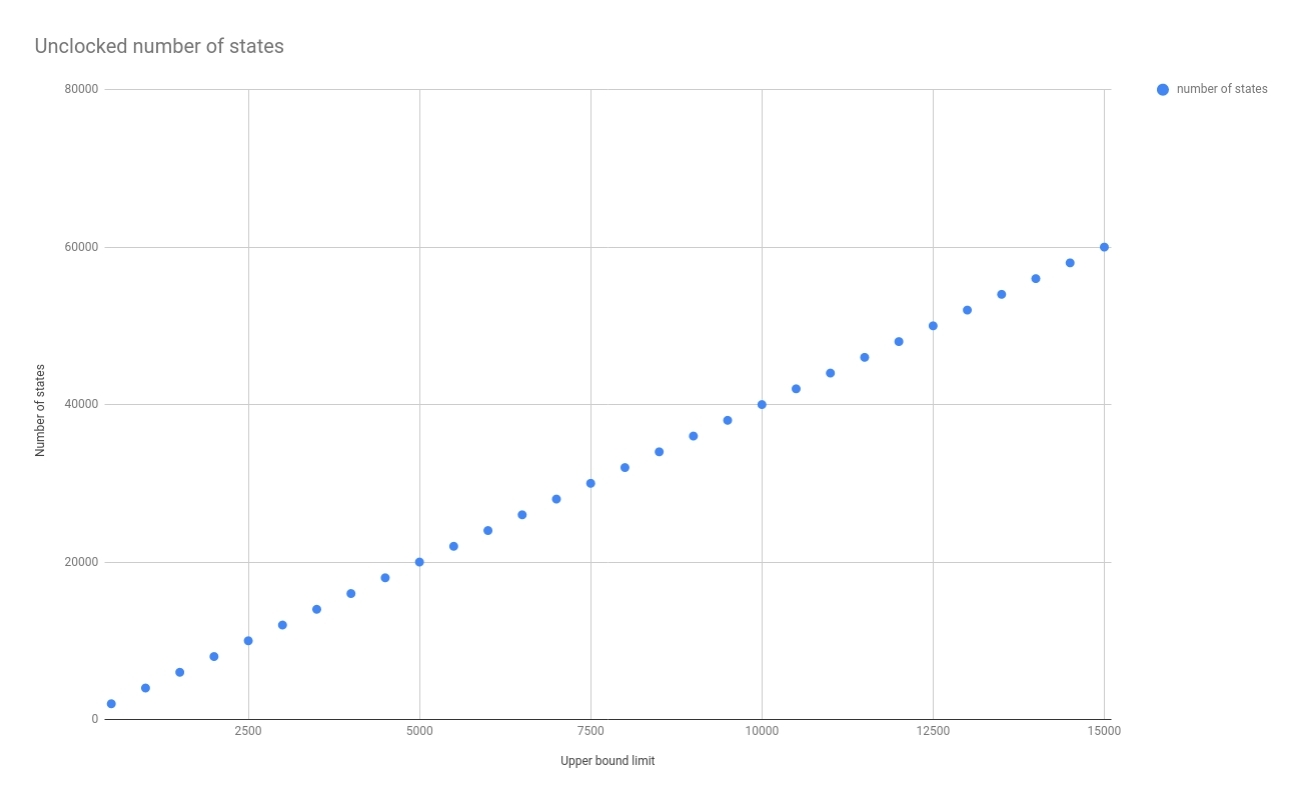
\includegraphics[width=0.98\textwidth]{./figures/temporary_graphs/unclocked_number_of_states.jpg}
\caption{Graph of the \texttt{number of visited states} property from the unclocked seven segments experiment.}
\label{fig:unclocked_states}
\end{figure}
\paragraph{Verification time}
In Figure \ref{fig:unclocked_verification} the \texttt{verification time} results can be seen. The graph represents the verification time in seconds for each increase in the input range. As can be seen the verification time increase exponentially with the input values. Since the number of states visited is increasing linearly it can seem odd that the verification time does not follow that same pattern. However, besides the refinement checking of the GLTS, which will increase with the number of states, FDR4 must compile the network and generate the GLTS. It is reasonable to expect that the larger the state space, the more effort for FDR4 to complete all the steps of the verification. Therefore these results are consistent with what could be expected.
\begin{figure}
    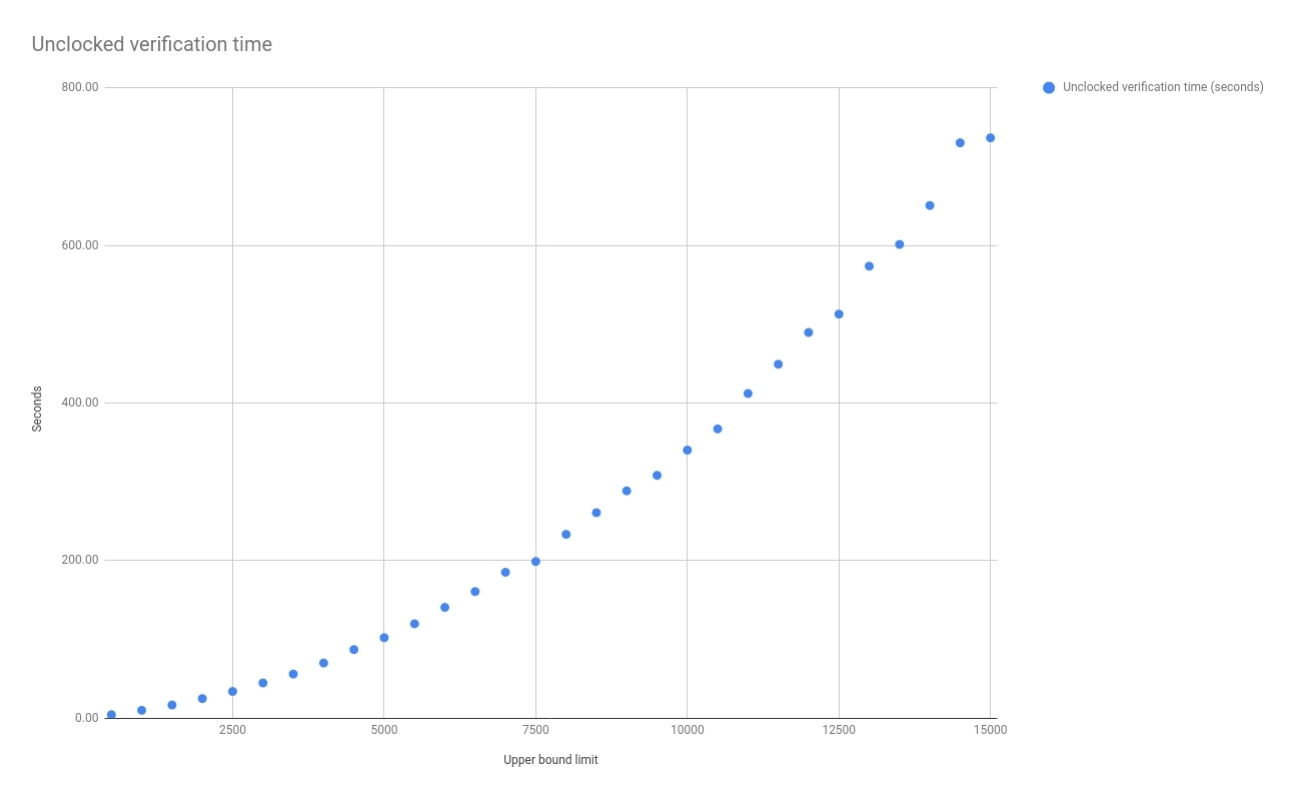
\includegraphics[width=0.98\textwidth]{./figures/temporary_graphs/unclocked_verification_time.jpg}
\caption{Graph of the \texttt{verification time} property from the unclocked seven segments experiment.}
\label{fig:unclocked_verification}
\end{figure}
\paragraph{Maximum resident set size}
The result from this property can be seen in Figure \ref{fig:unclocked_resident_size}. These results are not fitted to a perfect line as well as the other two experiment properties. It is clear that the amount of memory used for the verification grows with an increase in the input range. It is also somewhat consistent until around 10000 in upper bound limit. This fluctuation could be caused by some internal structure in FDR4 or it could be a result of other processes running on the machine that is running the verification. Unfortunately, FDR4 does not provide a lot of information about the internal workings and so it can be very difficult to examine these results further. However, the results are overall consistent with the results from both \texttt{number of visited states} and \texttt{verification time}.
\begin{figure}
    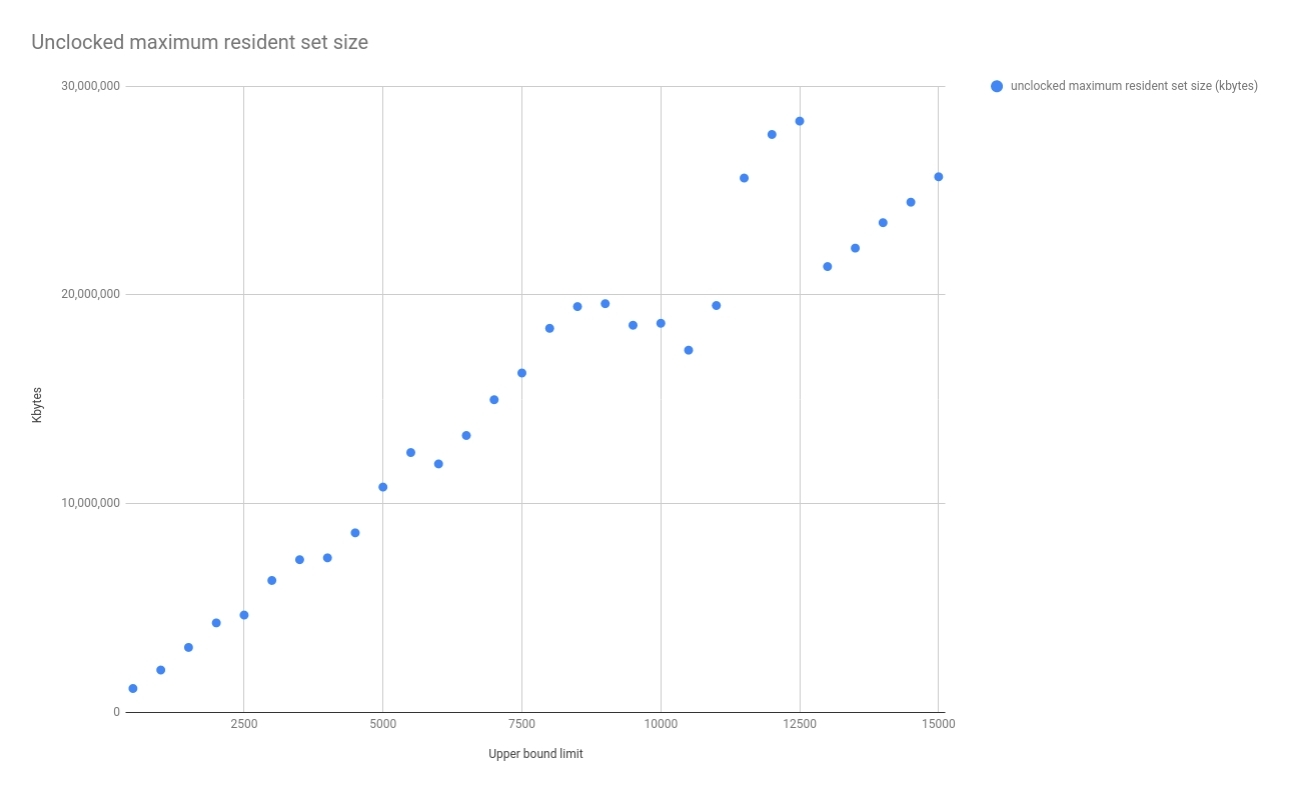
\includegraphics[width=0.98\textwidth]{./figures/temporary_graphs/unclocked_maximum_resident_set_size.jpg}
\caption{Graph of the \texttt{maximum resident set size} property from the unclocked seven segments experiment.}
\label{fig:unclocked_resident_size}
\end{figure}

\subsection{Clocked Experiment}
The full code for the clocked seven segments display example can be seen in Listing \ref{lst:cspm} in Appendix. %TODO: Figure out how this should be presented. One appendix or several?
As in the unclocked seven segments display example, the clocked example also consists of three \texttt{time} processes with associated monitor processes.
In order to make the clocked seven segment experiment equivalent with the unclocked seven segments example, the \texttt{Clock} process in the clocked network only verifies one clock cycle and therefore the two networks should be equivalent in the verification.
\paragraph{Number of visited states}
In Figure \ref{fig:clocked_states}the results of the clocked \texttt{number of visited states} property can be seen for each \texttt{time} verification. As can be seen, they differ quite a lot from each other. The \texttt{number of visited states} property for \texttt{hour} seems to increase every 3600 input increase, and since there are 3600 seconds in one hour, this means that every time the input represents an extra hour, the number of states increase. The \texttt{number of visited states} for \texttt{minutes} increase linearly until exactly 5339 and then stays at 134 for the rest of the verifications. It is very clear from this result that the number of states reaches its maximum when the input range represents the maximum amount of minutes. The input range \{0..5339\} represents 59 minutes which is maximum. The \texttt{number of visited states} for \texttt{seconds} is constant at 134, however if the input range was decreased to \{0..59\} the same result could be seen as with the \texttt{minutes} graph. These results make it clear that FDR4 is able to decrease the number of states to the number of \texttt{hours}, \texttt{minutes} and \texttt{seconds} represented by the input.
\begin{figure}
    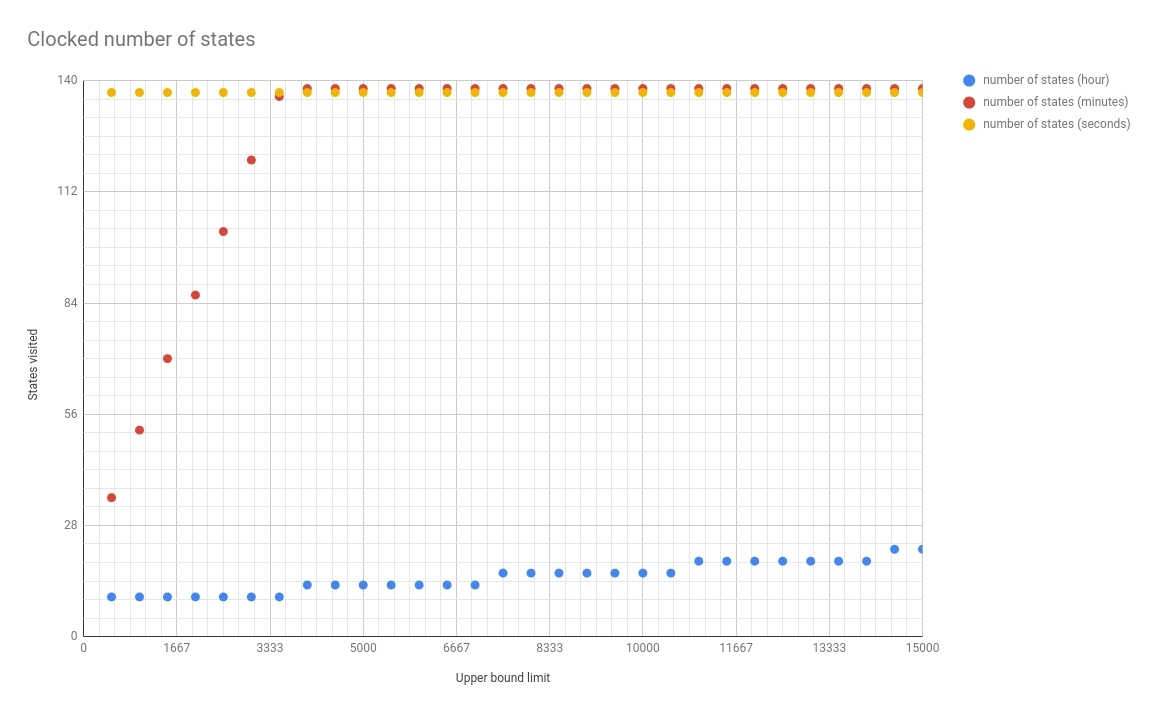
\includegraphics[width=0.98\textwidth]{./figures/temporary_graphs/clocked_number_of_states.jpg}
\caption{Graphs of the three \texttt{number of visited states} properties from the clocked seven segments experiment.}
\label{fig:clocked_states}
\end{figure}
\paragraph{Verification time}
In Figure \ref{fig:clocked_verification} the clocked \texttt{verification time}
results can be seen.
This graph is very similar to the \texttt{verification time} results for the unclocked experiment but with a slightly different increase. However, the values also increase exponentially with the input which, as explained above, is to be expected. What is important to notice is that even though the graph is similar to the unclocked \texttt{verification time} graph, the number of seconds are very different than in the first experiment. The reason for this is probably the decrease in \texttt{number of visited states} which will be discussed further below.
\begin{figure}
    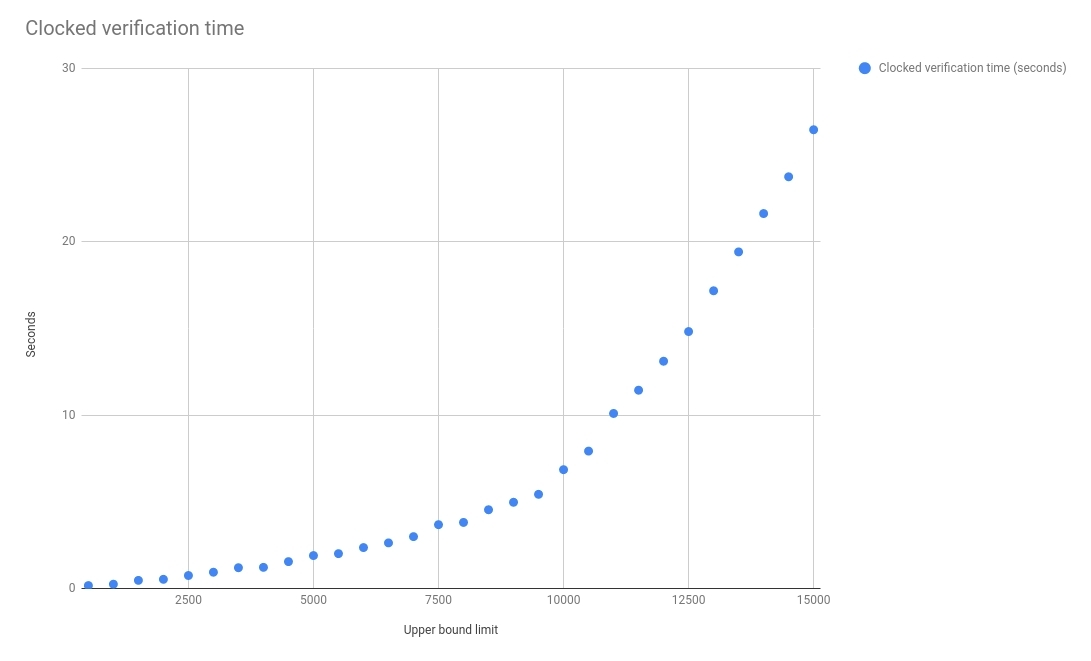
\includegraphics[width=0.98\textwidth]{./figures/temporary_graphs/clocked_verification_time.jpg}
\caption{Graph of the \texttt{verification time} property from the clocked seven segments experiment.}
\label{fig:clocked_verification}
\end{figure}
\paragraph{Maximum resident set size}
Figure \ref{fig:clocked_resident_size} shows the clocked \texttt{maximum resident set size}. This graph shows the same situation as the \texttt{verification time} graph. The graph is similar to that of the unclocked \texttt{maximum resident set size} with a slightly more flattened increase and not nearly as much fluctuation. The big difference with this graph is again the low values compared to the unclocked \texttt{maximum resident set size} values. This is also discussed further below.
\begin{figure}
    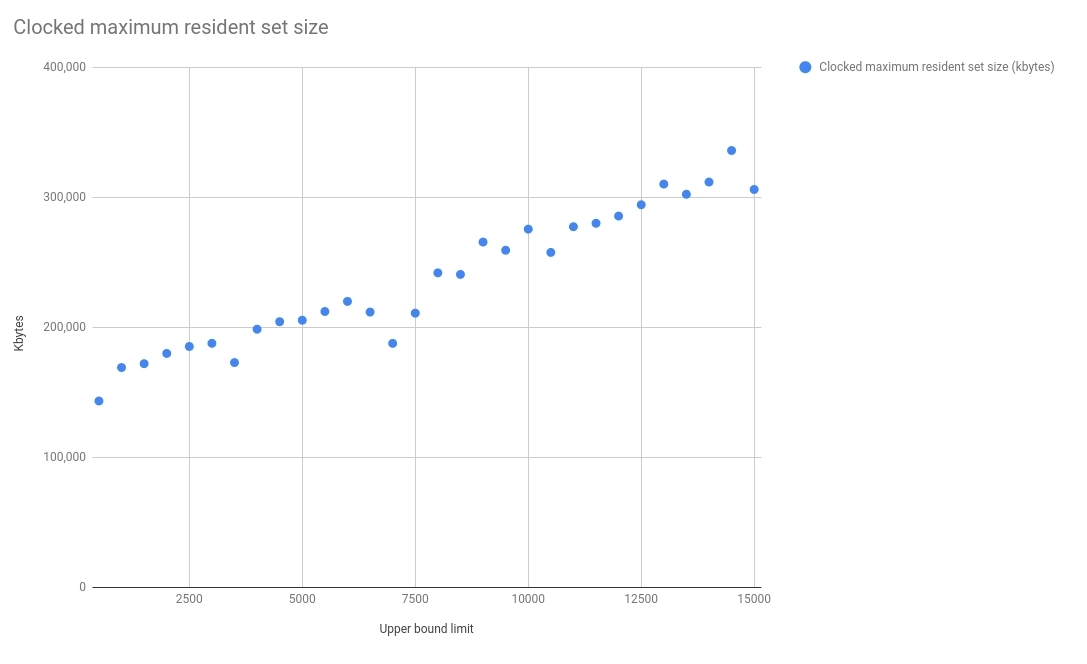
\includegraphics[width=0.98\textwidth]{./figures/temporary_graphs/clocked_maximum_resident_set_size.jpg}
\caption{Graph of the \texttt{maximum resident set size} property from the clocked seven segments experiment.}
\label{fig:clocked_resident_size}
\end{figure}
\subsection{Results}
% TODO when I know I can use this example
As explained above, the \texttt{number of visited states} property from the unclocked seven segments experiment showed to be equal for all three \texttt{time} verifications whereas, for the clocked experiment, the \texttt{number of visited states} varied between the three verifications. Figure \ref{fig:combined_states} represents all four graphs, however, only two can be seen. %TODO: Make sure the actual graph used also looks like this.
The reason for this is that the values of the clocked \texttt{number of visited states} are so much lower than the unclocked results that they cannot be shown separately in the graph. \\

In Figure \ref{fig:combined_verification} the combined \texttt{verification time} graph can be seen. Here, the difference also shows very clearly. The clocked experiment verifies much faster than the unclocked. Again it is not possible to display the actual values of the clocked version in the graph because they are too low to be displayed properly. The same case can be seen in Figure \ref{fig:combined_resident_size} which represents the combined \texttt{maximum resident set size}. \\

Both \texttt{verification time} and \texttt{resident set size} seem to be affected by the \texttt{number of visited states} property. This is evident because the
\texttt{number of visited states} is the only internal FDR4 property of the experiment. Unfortunately, it can be quite difficult to investigate why the clocked experiment performs so much better than the unclocked. When looking at the trace of both networks within FDR4, both verify the full input range, as expected. The visualiser ProBE also shows equivalent traces and the two networks behave identically on failures. The only difference between the two networks is that in the clocked system all processes are recursive and synchronise together before continuing. The unclocked processes will always terminate after one clock cycle. However, since the clocked network only simulates one clock cycle, the two networks should still be equivalent. These differences do not affect the actual values verified or the result of the verification. As previously stated when introducing the clocked version of TAPS in Chapter \ref{chap:clock} the increase in complexity might increase the verification time in FDR4, but in this case, it is the opposite. \\

As the two networks seem equivalent in both input range and verification, the reason for the difference in performance might lie in what the \texttt{number of visited states} property shows. It might be that FDR4 is able to compress the state space in the clocked experiment while not being able to perform the same compression in the unclocked experiment. \\

The FDR4 tool provides a machine structure viewer which can provide information about how FDR4 represents the processes and how effective the compression is. When looking at the two different results from FDR4 it becomes clear why the clocked experiment performs so much better than the unclocked experiment. In Figure \ref{fig:unclocked_compression} and Figure \ref{fig:clocked_compression}, the output of the machine structure viewer can be seen. In the unclocked result in Figure \ref{fig:unclocked_compression} the unclocked network
\texttt{N\_hours} is represented by a high-level machine with 12 formats, 77 rules, and 34 leaf machines. A high-level machine means a process with subprocesses and the only information needed about formats and rules are that the more there are, the more complex the machine. \\

Because all events are hidden in the network, as explained in Chapter \ref{chap:design}, the subprocesses are \texttt{Unknown}. The second to last line shows that the compression algorithm \texttt{sbisim} have been applied to \texttt{Hours(0)} but it also shows that it was not able to reduce the number of states or transitions. \\

Figure \ref{fig:clocked_compression} represents the clocked network and, as can be seen, the \texttt{N\_hours} process includes compression information. It provides an estimate that the reduced machine is around 17\% the size of the original machine. On the second to last line, it can be seen that the \texttt{sbisim} compression algorithm is not applied to \texttt{Hours(0)} as in the unclocked experiment, but to \texttt{Hours(..)}. The \texttt{sbisim} compression algorithm is able to compress the state space from 36 states to 6 states. It clearly shows that because FDR4 is able to perform compression on the clocked system, the performance also increases dramatically.\\

It is quite surprising that the clocked experiment have such a drastic difference and that it actually performs better than the unclocked version. As the network increase in complexity the state space should also increase, and it is only because of the compression that the clocked version performs so well. It is, however, not possible to learn exactly why FDR4 is able to perform compression on the clocked network and not on the unclocked. There is a lot of different aspects the way FDR4 structures the network and generate the GLTS. Somehow the clocked network is structured in a way that fits better into the compression algorithm than the unclocked network.
\begin{figure}
    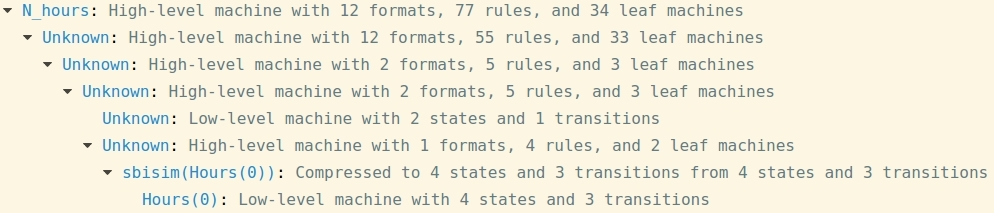
\includegraphics[width=0.98\textwidth]{./figures/unclocked_compression.jpg}
\caption{Screen dump of the results of the unclocked network in the FDR4 machine structure viewer.}
\label{fig:unclocked_compression}
\end{figure}
\begin{figure}
    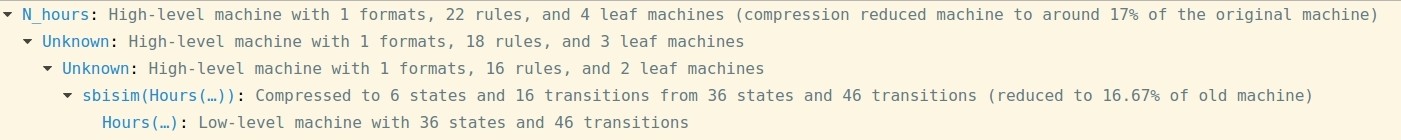
\includegraphics[width=0.98\textwidth]{./figures/clocked_compression.jpg}
\caption{Screen dump of the results of the clocked network in the FDR4 machine structure viewer.}
\label{fig:clocked_compression}
\end{figure}

\begin{figure}
    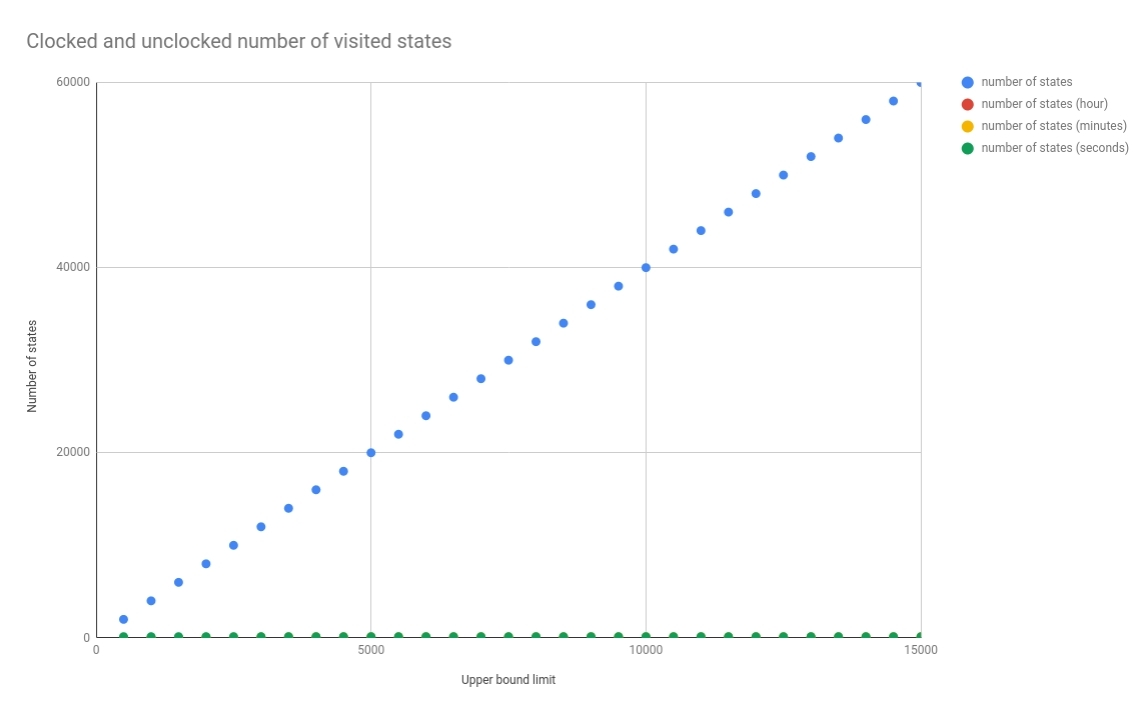
\includegraphics[width=0.98\textwidth]{./figures/temporary_graphs/combined_number_of_states.jpg}
\caption{Graphs of the \texttt{number of states} properties combined from both the unclocked and clocked seven segments experiment.}
\label{fig:combined_states}
\end{figure}

\begin{figure}
    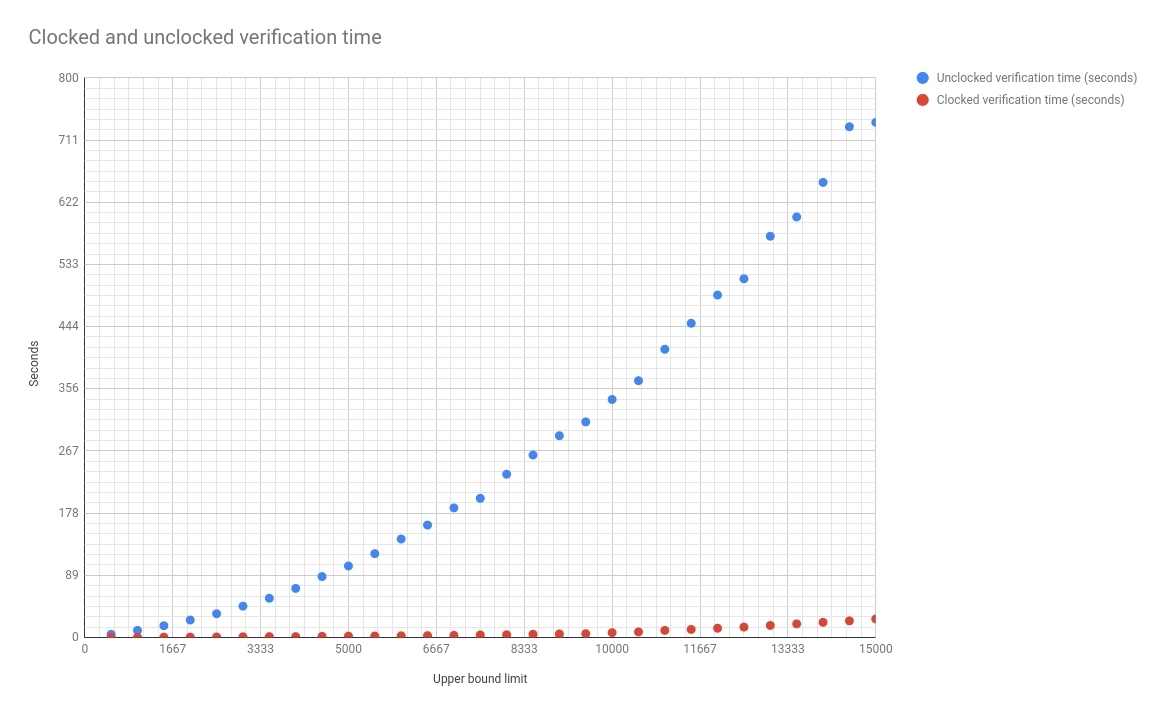
\includegraphics[width=0.98\textwidth]{./figures/temporary_graphs/combined_verification_time.jpg}
\caption{Graphs of the \texttt{verification time} properties combined from both the unclocked and clocked seven segments experiment.}
\label{fig:combined_verification}
\end{figure}

\begin{figure}
    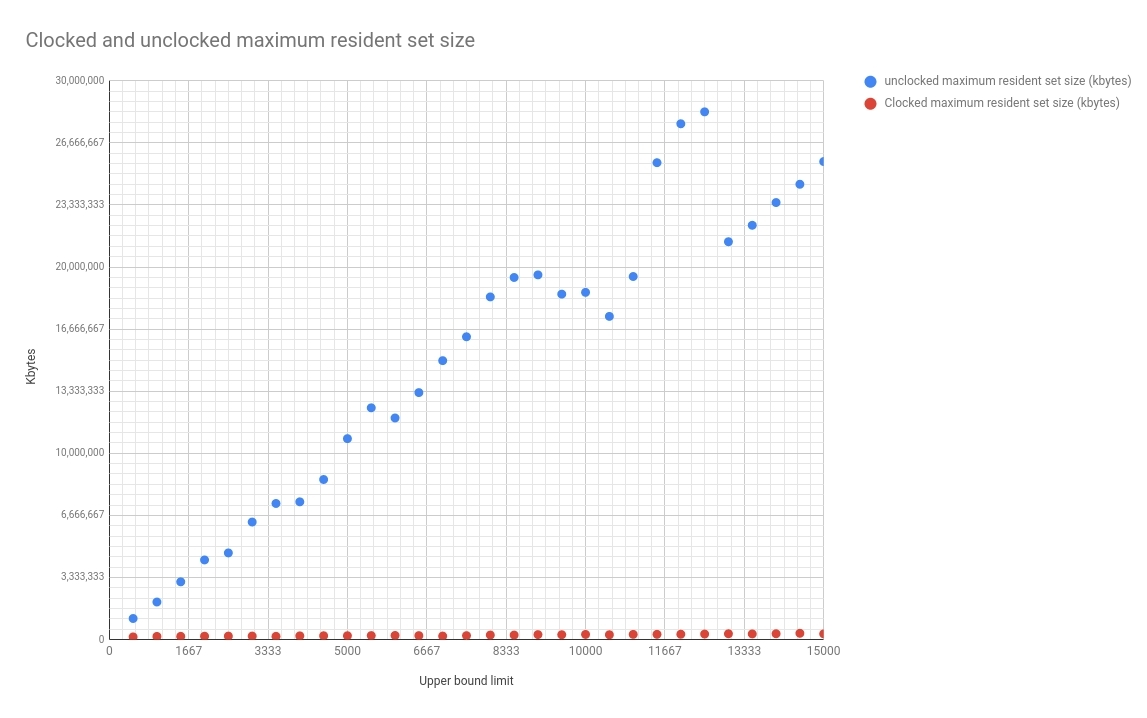
\includegraphics[width=0.98\textwidth]{./figures/temporary_graphs/combined_maximum_resident_set_size.jpg}
\caption{Graphs of the \texttt{maximum resident size set} properties combined from both the unclocked and clocked seven segments experiment.}
\label{fig:combined_resident_size}
\end{figure}




% TODO: I should also still mention something about how the increase in number of processes was or was not feasible.



\newpage
\section{How to use TAPS}
The required dependencies for generating the ANTLR4 parser, running TAPS and verification with FDR4 are listed below:
\begin{itemize}
    \item ANTLR4
    \item Python 2.7
    \item ANTLR Python runtime
    \item FDR4
\end{itemize}

ANTLR4 and FDR4 can both be downloaded from their websites where installation instructions are also provided.
The ANTLR4 project can be found at \url{https://www.antlr.org/} and the FDR4 Project at \url{https://www.cs.ox.ac.uk/projects/fdr/}.\\
It is also necessary to download the ANTLR4 Python runtime from \url{https://pypi.org/project/antlr4-python2-runtime/}.

Assuming that an ANTLR4 alias has been created as the ANTLR4 installation suggest, the parser and lexer can be generated with ANTLR4 using the command: {\ttfamily antlr4 -Dlanguage=Python2 - visitor -no-listener Smeil.g4.}
This will create all the required parser and lexer files as well as the visitor methods. This step is only necessary if the .g4 grammar file has been modified.\\

When the ANTLR4 files have been generated TAPS can be used directly with a well-formed SMEIL program with the command: {\ttfamily python taps.py input.sme output.csp}. The system requires both an input file as well as an output file. If the output file does not exist it will be created by TAPS. \\

The resulting \cspm{} file can be verified in FDR either by the command line tool or by the FDR4 tool which is a graphical tool. The command line tool can be used by the command \texttt{refines output.csp}. There are several options to adjust the output of the command. The FDR4 command line tool is mostly used to quickly check if a network passes the verification because it is difficult to navigate the counterexamples. The FDR4 graphical tool provides a better visualisation of counterexamples and the ProBE visualiser can be called directly from the FDR graphical tool.

